% Generated by Sphinx.
\def\sphinxdocclass{report}
\documentclass[letterpaper,11pt,openany,oneside]{sphinxmanual}
\usepackage[utf8]{inputenc}
\DeclareUnicodeCharacter{00A0}{\nobreakspace}
\usepackage{cmap}
\usepackage[T1]{fontenc}
\usepackage[british]{babel}
\usepackage{times}
\usepackage[Bjarne]{fncychap}
\usepackage{longtable}
\usepackage{sphinx}
\usepackage{multirow}
\usepackage{amsmath,amssymb}


\title{oBB Documentation}
\date{19 November, 2014}
\release{0.7b}
\author{J. M. Fowkes}
\newcommand{\sphinxlogo}{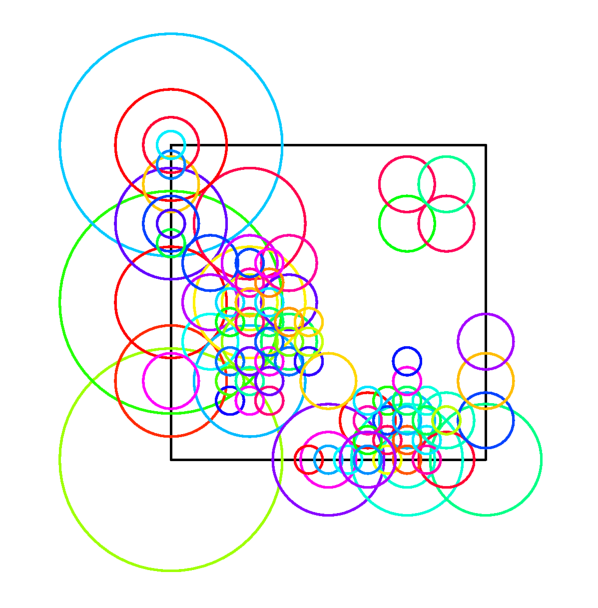
\includegraphics{p1.pdf}\par}
\renewcommand{\releasename}{Release}
\makeindex

\makeatletter
\def\PYG@reset{\let\PYG@it=\relax \let\PYG@bf=\relax%
    \let\PYG@ul=\relax \let\PYG@tc=\relax%
    \let\PYG@bc=\relax \let\PYG@ff=\relax}
\def\PYG@tok#1{\csname PYG@tok@#1\endcsname}
\def\PYG@toks#1+{\ifx\relax#1\empty\else%
    \PYG@tok{#1}\expandafter\PYG@toks\fi}
\def\PYG@do#1{\PYG@bc{\PYG@tc{\PYG@ul{%
    \PYG@it{\PYG@bf{\PYG@ff{#1}}}}}}}
\def\PYG#1#2{\PYG@reset\PYG@toks#1+\relax+\PYG@do{#2}}

\expandafter\def\csname PYG@tok@vc\endcsname{\def\PYG@tc##1{\textcolor[rgb]{0.73,0.38,0.84}{##1}}}
\expandafter\def\csname PYG@tok@nd\endcsname{\let\PYG@bf=\textbf\def\PYG@tc##1{\textcolor[rgb]{0.33,0.33,0.33}{##1}}}
\expandafter\def\csname PYG@tok@nc\endcsname{\let\PYG@bf=\textbf\def\PYG@tc##1{\textcolor[rgb]{0.05,0.52,0.71}{##1}}}
\expandafter\def\csname PYG@tok@nt\endcsname{\let\PYG@bf=\textbf\def\PYG@tc##1{\textcolor[rgb]{0.02,0.16,0.45}{##1}}}
\expandafter\def\csname PYG@tok@mo\endcsname{\def\PYG@tc##1{\textcolor[rgb]{0.13,0.50,0.31}{##1}}}
\expandafter\def\csname PYG@tok@bp\endcsname{\def\PYG@tc##1{\textcolor[rgb]{0.00,0.44,0.13}{##1}}}
\expandafter\def\csname PYG@tok@nb\endcsname{\def\PYG@tc##1{\textcolor[rgb]{0.00,0.44,0.13}{##1}}}
\expandafter\def\csname PYG@tok@nv\endcsname{\def\PYG@tc##1{\textcolor[rgb]{0.73,0.38,0.84}{##1}}}
\expandafter\def\csname PYG@tok@se\endcsname{\let\PYG@bf=\textbf\def\PYG@tc##1{\textcolor[rgb]{0.25,0.44,0.63}{##1}}}
\expandafter\def\csname PYG@tok@ne\endcsname{\def\PYG@tc##1{\textcolor[rgb]{0.00,0.44,0.13}{##1}}}
\expandafter\def\csname PYG@tok@ss\endcsname{\def\PYG@tc##1{\textcolor[rgb]{0.32,0.47,0.09}{##1}}}
\expandafter\def\csname PYG@tok@go\endcsname{\def\PYG@tc##1{\textcolor[rgb]{0.20,0.20,0.20}{##1}}}
\expandafter\def\csname PYG@tok@c1\endcsname{\let\PYG@it=\textit\def\PYG@tc##1{\textcolor[rgb]{0.25,0.50,0.56}{##1}}}
\expandafter\def\csname PYG@tok@vi\endcsname{\def\PYG@tc##1{\textcolor[rgb]{0.73,0.38,0.84}{##1}}}
\expandafter\def\csname PYG@tok@s1\endcsname{\def\PYG@tc##1{\textcolor[rgb]{0.25,0.44,0.63}{##1}}}
\expandafter\def\csname PYG@tok@sb\endcsname{\def\PYG@tc##1{\textcolor[rgb]{0.25,0.44,0.63}{##1}}}
\expandafter\def\csname PYG@tok@kc\endcsname{\let\PYG@bf=\textbf\def\PYG@tc##1{\textcolor[rgb]{0.00,0.44,0.13}{##1}}}
\expandafter\def\csname PYG@tok@gi\endcsname{\def\PYG@tc##1{\textcolor[rgb]{0.00,0.63,0.00}{##1}}}
\expandafter\def\csname PYG@tok@ow\endcsname{\let\PYG@bf=\textbf\def\PYG@tc##1{\textcolor[rgb]{0.00,0.44,0.13}{##1}}}
\expandafter\def\csname PYG@tok@kt\endcsname{\def\PYG@tc##1{\textcolor[rgb]{0.56,0.13,0.00}{##1}}}
\expandafter\def\csname PYG@tok@mh\endcsname{\def\PYG@tc##1{\textcolor[rgb]{0.13,0.50,0.31}{##1}}}
\expandafter\def\csname PYG@tok@na\endcsname{\def\PYG@tc##1{\textcolor[rgb]{0.25,0.44,0.63}{##1}}}
\expandafter\def\csname PYG@tok@ni\endcsname{\let\PYG@bf=\textbf\def\PYG@tc##1{\textcolor[rgb]{0.84,0.33,0.22}{##1}}}
\expandafter\def\csname PYG@tok@ge\endcsname{\let\PYG@it=\textit}
\expandafter\def\csname PYG@tok@sr\endcsname{\def\PYG@tc##1{\textcolor[rgb]{0.14,0.33,0.53}{##1}}}
\expandafter\def\csname PYG@tok@si\endcsname{\let\PYG@it=\textit\def\PYG@tc##1{\textcolor[rgb]{0.44,0.63,0.82}{##1}}}
\expandafter\def\csname PYG@tok@kp\endcsname{\def\PYG@tc##1{\textcolor[rgb]{0.00,0.44,0.13}{##1}}}
\expandafter\def\csname PYG@tok@sx\endcsname{\def\PYG@tc##1{\textcolor[rgb]{0.78,0.36,0.04}{##1}}}
\expandafter\def\csname PYG@tok@w\endcsname{\def\PYG@tc##1{\textcolor[rgb]{0.73,0.73,0.73}{##1}}}
\expandafter\def\csname PYG@tok@o\endcsname{\def\PYG@tc##1{\textcolor[rgb]{0.40,0.40,0.40}{##1}}}
\expandafter\def\csname PYG@tok@k\endcsname{\let\PYG@bf=\textbf\def\PYG@tc##1{\textcolor[rgb]{0.00,0.44,0.13}{##1}}}
\expandafter\def\csname PYG@tok@gt\endcsname{\def\PYG@tc##1{\textcolor[rgb]{0.00,0.27,0.87}{##1}}}
\expandafter\def\csname PYG@tok@mf\endcsname{\def\PYG@tc##1{\textcolor[rgb]{0.13,0.50,0.31}{##1}}}
\expandafter\def\csname PYG@tok@err\endcsname{\def\PYG@bc##1{\setlength{\fboxsep}{0pt}\fcolorbox[rgb]{1.00,0.00,0.00}{1,1,1}{\strut ##1}}}
\expandafter\def\csname PYG@tok@s\endcsname{\def\PYG@tc##1{\textcolor[rgb]{0.25,0.44,0.63}{##1}}}
\expandafter\def\csname PYG@tok@gd\endcsname{\def\PYG@tc##1{\textcolor[rgb]{0.63,0.00,0.00}{##1}}}
\expandafter\def\csname PYG@tok@gu\endcsname{\let\PYG@bf=\textbf\def\PYG@tc##1{\textcolor[rgb]{0.50,0.00,0.50}{##1}}}
\expandafter\def\csname PYG@tok@nn\endcsname{\let\PYG@bf=\textbf\def\PYG@tc##1{\textcolor[rgb]{0.05,0.52,0.71}{##1}}}
\expandafter\def\csname PYG@tok@cp\endcsname{\def\PYG@tc##1{\textcolor[rgb]{0.00,0.44,0.13}{##1}}}
\expandafter\def\csname PYG@tok@no\endcsname{\def\PYG@tc##1{\textcolor[rgb]{0.38,0.68,0.84}{##1}}}
\expandafter\def\csname PYG@tok@sc\endcsname{\def\PYG@tc##1{\textcolor[rgb]{0.25,0.44,0.63}{##1}}}
\expandafter\def\csname PYG@tok@nf\endcsname{\def\PYG@tc##1{\textcolor[rgb]{0.02,0.16,0.49}{##1}}}
\expandafter\def\csname PYG@tok@kn\endcsname{\let\PYG@bf=\textbf\def\PYG@tc##1{\textcolor[rgb]{0.00,0.44,0.13}{##1}}}
\expandafter\def\csname PYG@tok@vg\endcsname{\def\PYG@tc##1{\textcolor[rgb]{0.73,0.38,0.84}{##1}}}
\expandafter\def\csname PYG@tok@mb\endcsname{\def\PYG@tc##1{\textcolor[rgb]{0.13,0.50,0.31}{##1}}}
\expandafter\def\csname PYG@tok@nl\endcsname{\let\PYG@bf=\textbf\def\PYG@tc##1{\textcolor[rgb]{0.00,0.13,0.44}{##1}}}
\expandafter\def\csname PYG@tok@gp\endcsname{\let\PYG@bf=\textbf\def\PYG@tc##1{\textcolor[rgb]{0.78,0.36,0.04}{##1}}}
\expandafter\def\csname PYG@tok@il\endcsname{\def\PYG@tc##1{\textcolor[rgb]{0.13,0.50,0.31}{##1}}}
\expandafter\def\csname PYG@tok@sh\endcsname{\def\PYG@tc##1{\textcolor[rgb]{0.25,0.44,0.63}{##1}}}
\expandafter\def\csname PYG@tok@kd\endcsname{\let\PYG@bf=\textbf\def\PYG@tc##1{\textcolor[rgb]{0.00,0.44,0.13}{##1}}}
\expandafter\def\csname PYG@tok@kr\endcsname{\let\PYG@bf=\textbf\def\PYG@tc##1{\textcolor[rgb]{0.00,0.44,0.13}{##1}}}
\expandafter\def\csname PYG@tok@m\endcsname{\def\PYG@tc##1{\textcolor[rgb]{0.13,0.50,0.31}{##1}}}
\expandafter\def\csname PYG@tok@cm\endcsname{\let\PYG@it=\textit\def\PYG@tc##1{\textcolor[rgb]{0.25,0.50,0.56}{##1}}}
\expandafter\def\csname PYG@tok@gs\endcsname{\let\PYG@bf=\textbf}
\expandafter\def\csname PYG@tok@s2\endcsname{\def\PYG@tc##1{\textcolor[rgb]{0.25,0.44,0.63}{##1}}}
\expandafter\def\csname PYG@tok@gh\endcsname{\let\PYG@bf=\textbf\def\PYG@tc##1{\textcolor[rgb]{0.00,0.00,0.50}{##1}}}
\expandafter\def\csname PYG@tok@sd\endcsname{\let\PYG@it=\textit\def\PYG@tc##1{\textcolor[rgb]{0.25,0.44,0.63}{##1}}}
\expandafter\def\csname PYG@tok@mi\endcsname{\def\PYG@tc##1{\textcolor[rgb]{0.13,0.50,0.31}{##1}}}
\expandafter\def\csname PYG@tok@c\endcsname{\let\PYG@it=\textit\def\PYG@tc##1{\textcolor[rgb]{0.25,0.50,0.56}{##1}}}
\expandafter\def\csname PYG@tok@cs\endcsname{\def\PYG@tc##1{\textcolor[rgb]{0.25,0.50,0.56}{##1}}\def\PYG@bc##1{\setlength{\fboxsep}{0pt}\colorbox[rgb]{1.00,0.94,0.94}{\strut ##1}}}
\expandafter\def\csname PYG@tok@gr\endcsname{\def\PYG@tc##1{\textcolor[rgb]{1.00,0.00,0.00}{##1}}}

\def\PYGZbs{\char`\\}
\def\PYGZus{\char`\_}
\def\PYGZob{\char`\{}
\def\PYGZcb{\char`\}}
\def\PYGZca{\char`\^}
\def\PYGZam{\char`\&}
\def\PYGZlt{\char`\<}
\def\PYGZgt{\char`\>}
\def\PYGZsh{\char`\#}
\def\PYGZpc{\char`\%}
\def\PYGZdl{\char`\$}
\def\PYGZhy{\char`\-}
\def\PYGZsq{\char`\'}
\def\PYGZdq{\char`\"}
\def\PYGZti{\char`\~}
% for compatibility with earlier versions
\def\PYGZat{@}
\def\PYGZlb{[}
\def\PYGZrb{]}
\makeatother

\renewcommand\PYGZsq{\textquotesingle}

\begin{document}

\maketitle
\tableofcontents
\phantomsection\label{index::doc}


\textbf{Release:} 0.7b

\textbf{Date:} 19 November, 2014

\textbf{Author:} \href{mailto:jaroslav.fowkes@ed.ac.uk}{J. M. Fowkes}

oBB is an algorithm for the parallel global optimization of functions with Lipchitz continuous gradient or Hessian.


\chapter{Installing oBB}
\label{install::doc}\label{install:installing-obb}\label{install:overlapping-branch-and-bound}

\section{Requirements}
\label{install:requirements}
oBB requires the following software to be installed:
\begin{itemize}
\item {} 
\href{http://www.python.org/}{Python 2.6/2.7 or Python 3}

\item {} 
A working implementation of MPI-2 (e.g. \href{http://www.open-mpi.org/}{OpenMPI} or \href{http://www.mpich.org/}{MPICH})

\end{itemize}

Additionally, the following python packages should be installed (these will be installed automatically if using \href{http://www.pip-installer.org/}{pip}, see {\hyperref[install:installation-using-pip]{Installation using pip}}):
\begin{itemize}
\item {} 
\href{http://www.numpy.org/}{NumPy 1.3.0 or higher}

\item {} 
\href{http://mpi4py.scipy.org/}{MPI for Python 1.3 or higher}

\item {} 
\href{http://cvxopt.org/}{CVXOPT 1.1.3 or higher}

\end{itemize}

Optionally, \href{http://www.matplotlib.org/}{matplotlib 1.1.0 or higher} may be manually installed for visualising the algorithm in 2D.


\section{Installation using pip}
\label{install:installation-using-pip}
For easy installation, use \href{http://www.pip-installer.org/}{pip} as root:
\begin{quote}

\begin{Verbatim}[commandchars=\\\{\}]
\PYG{n+nv}{\PYGZdl{} }\PYG{o}{[}sudo\PYG{o}{]} pip install \PYGZhy{}\PYGZhy{}pre obb
\end{Verbatim}
\end{quote}

or alternatively \emph{easy\_install}:
\begin{quote}

\begin{Verbatim}[commandchars=\\\{\}]
\PYG{n+nv}{\PYGZdl{} }\PYG{o}{[}sudo\PYG{o}{]} easy\PYGZus{}install obb
\end{Verbatim}
\end{quote}

If you do not have root privileges or you want to install oBB for your private use, you can use:
\begin{quote}

\begin{Verbatim}[commandchars=\\\{\}]
\PYG{n+nv}{\PYGZdl{} }pip install \PYGZhy{}\PYGZhy{}pre \PYGZhy{}\PYGZhy{}user obb
\end{Verbatim}
\end{quote}

which will install oBB in your home directory.

Note that if an older install of oBB is present on your system you can use:
\begin{quote}

\begin{Verbatim}[commandchars=\\\{\}]
\PYG{n+nv}{\PYGZdl{} }\PYG{o}{[}sudo\PYG{o}{]} pip install \PYGZhy{}\PYGZhy{}pre \PYGZhy{}\PYGZhy{}upgrade obb
\end{Verbatim}
\end{quote}

to upgrade oBB to the latest version.


\section{Manual installation}
\label{install:manual-installation}
Alternatively, you can download the source code and unpack as follows:
\begin{quote}

\begin{Verbatim}[commandchars=\\\{\}]
\PYG{n+nv}{\PYGZdl{} }wget http://pypi.python.org/packages/source/o/oBB/oBB\PYGZhy{}X.X.tar.gz
\PYG{n+nv}{\PYGZdl{} }tar \PYGZhy{}xzvf oBB\PYGZhy{}X.X.tar.gz
\PYG{n+nv}{\PYGZdl{} }\PYG{n+nb}{cd }oBB\PYGZhy{}X.X
\end{Verbatim}
\end{quote}

and then build and install manually using:
\begin{quote}

\begin{Verbatim}[commandchars=\\\{\}]
\PYG{n+nv}{\PYGZdl{} }python setup.py build
\PYG{n+nv}{\PYGZdl{} }\PYG{o}{[}sudo\PYG{o}{]} python setup.py install
\end{Verbatim}
\end{quote}

If you do not have root privileges or you want to install oBB for your private use, you can use:
\begin{quote}

\begin{Verbatim}[commandchars=\\\{\}]
\PYG{n+nv}{\PYGZdl{} }python setup.py install \PYGZhy{}\PYGZhy{}user
\end{Verbatim}
\end{quote}

instead.


\section{Testing}
\label{install:testing}
oBB includes a command line test script to check that the installation was successfull. To run the test simply type the following into your shell:
\begin{quote}

\begin{Verbatim}[commandchars=\\\{\}]
\PYG{n+nv}{\PYGZdl{} }test\PYGZus{}obb
\end{Verbatim}
\end{quote}

This will run oBB using MPI on one processor core for a simple 2D sum of sines problem (see Example of Use).

Note that if using the MPICH implementation of MPI you first need to start an mpd daemon in the background:
\begin{quote}

\begin{Verbatim}[commandchars=\\\{\}]
\PYG{n+nv}{\PYGZdl{} }mpd \PYG{p}{\PYGZam{}}
\end{Verbatim}
\end{quote}

but this is not necessary for other MPI implementations, e.g. OpenMPI.


\section{Uninstallation}
\label{install:uninstallation}
If oBB was installed using \href{http://www.pip-installer.org/}{pip} you can uninstall as follows:
\begin{quote}

\begin{Verbatim}[commandchars=\\\{\}]
\PYG{n+nv}{\PYGZdl{} }\PYG{o}{[}sudo\PYG{o}{]} pip uninstall obb
\end{Verbatim}
\end{quote}

If oBB was installed manually you have to remove the installed files by hand (located in your python site-packages directory).


\chapter{User Guide}
\label{userguide::doc}\label{userguide:user-guide}
This section describes the main interface to oBB and how to use it.


\section{Global Optimization}
\label{userguide:global-optimization}
oBB is designed to solve the global optimization problem
\begin{quote}
\begin{gather}
\begin{split}&\min_{x \in \mathbb{R}^n} f(x) \\
\text{s.t. } \; &l \le x \le u \\
\text{and } \;  &Ax \le b \\
                &Ex = d\end{split}\notag
\end{gather}\end{quote}

where the objective function \(f\) has Lipschitz continuous gradient or Hessian. oBB does not need to know the Lipschitz constants explicitly, it merely requires the user to supply elementwise bounds on the Hessian or derivative tensor of the objective function (see {\hyperref[userguide:how-to-use-obb]{How to use oBB}}). The linear inequality constraints \(Ax \le b\) and equality constraints \(Ex = d\) are optional but the bound constraints \(l \le x \le u\) are required.

oBB uses local first or second order Taylor type approximations over balls within a parallel branch and bound framework. As with all branch and bound algorithms, the curse of dimensionality limits its use to low dimensional problems. The choice of whether to use first or second order approximations is down to the user  (see {\hyperref[userguide:how-to-use-obb]{How to use oBB}}).

For an in-depth technical description of the algorithm see the tech-report {\hyperref[userguide:cfg2013]{{[}CFG2013{]}}} and the paper {\hyperref[userguide:fgf2013]{{[}FGF2013{]}}}.


\section{How to use oBB}
\label{userguide:how-to-use-obb}
oBB requires the user to write a python script file that defines the functions and parameters necessary to solve the global optimization problem and then passes them to the main \textbf{obb} function (see {\hyperref[userguide:example-of-use]{Example of Use}}). The necessary functions are determined by the choice of a first or second order approximation model. The following approximation models can be passed to oBB's \textbf{obb} function using the \textbf{mod} argument (see {\hyperref[userguide:cfg2013]{{[}CFG2013{]}}} for details):
\begin{itemize}
\item {} 
First order models: \textbf{`q'} - norm based,  \textbf{`g'}, \textbf{`Hz'}, \textbf{`lbH'}, \textbf{`E0'}, \textbf{`Ediag'} - minimum eigenvalue based

\item {} 
Second order models: \textbf{`c'} - norm based, \textbf{`gc'} - minimum eigenvalue based

\end{itemize}

If using a first order model, the user is required to write the following functions:
\begin{itemize}
\item {} 
\textbf{f(x)} - returns objective function \(f\) at point \(x\) (scalar)

\item {} 
\textbf{g(x)} - returns gradient \(\nabla_x f\) of objective function at \(x\) (numpy 1D-array)

\end{itemize}

along with the bounding function:
\begin{itemize}
\item {} 
\textbf{bndH(l,u)} - returns two numpy 2D-arrays of elementwise lower and upper bounds on the Hessian \(\nabla_{xx} f\) of the objective function over \([l,u]\)

\end{itemize}

For a second order model the user is additionally required to write the function:
\begin{itemize}
\item {} 
\textbf{H(x)} - returns Hessian \(\nabla_{xx} f\) of objective function at \(x\) (numpy 2D-array)

\end{itemize}

and rather than \textbf{bndH} the bounding function:
\begin{itemize}
\item {} 
\textbf{bndT(l,u)} - returns two numpy 3D-arrays of elementwise lower and upper bounds on the derivative tensor \(\nabla_{xxx} f\) of the objective function over \([l,u]\)

\end{itemize}

The type of parallel branch and bound algorithm to use should be passed to oBB's \textbf{obb} function using the \textbf{alg} argument and can be one of the following (see {\hyperref[userguide:cfg2013]{{[}CFG2013{]}}} for details):
\begin{itemize}
\item {} 
\textbf{`T1'} - bounds in parallel

\item {} 
\textbf{`T2\_individual'}, \textbf{`T2\_synchronised'} - tree in parallel

\end{itemize}

See {\hyperref[userguide:example-of-use]{Example of Use}} for an in-depth worked example in python.


\section{Optional Arguments}
\label{userguide:optional-arguments}
oBB allows the user to specify several optional arguments that control the behaviour of the algorithm:
\begin{itemize}
\item {} 
\textbf{tol} - objective function tolerance (e.g. \textbf{1e-2}, the default)

\item {} 
\textbf{toltype} - tolerance type (\textbf{`r'} - relative {[}default{]}, \textbf{`a'} - absolute)

\item {} 
\textbf{countf} - count objective function evaluations (\textbf{0} - off, \textbf{1} - on {[}default{]})

\item {} 
\textbf{countsp} - count subproblem evaluations (\textbf{0} - off, \textbf{1} - on {[}default{]})

\end{itemize}

and if \href{http://www.matplotlib.org/}{matplotlib} is installed:
\begin{itemize}
\item {} 
\textbf{vis} - visualisation of the algorithm in 2D (\textbf{0} - off {[}default{]}, \textbf{1} - on)

\end{itemize}

Note that the inequality constraint arguments \(A, b\) and  equality constraint arguments \(E, d\) are also optional as the optimization problem is only required to be bound constrained.

The user can also specify the QP solver that the algorithm calls to obtain feasible upper bounds (see {\hyperref[userguide:cfg2013]{{[}CFG2013{]}}} for details). At present the user can choose from \href{http://cvxopt.org/}{CVXOPT's qp solver} or the \href{http://github.com/mpy/PyQuadProg/}{QuadProg++ solver} using the optional argument:
\begin{itemize}
\item {} 
\textbf{qpsolver} - QP solver to use (\textbf{`cvxopt'} - CVXOPT's qp {[}default{]}, \textbf{`quadprog'} - QuadProg++)

\end{itemize}

Note that the QuadProg++ solver is faster as it is written in C++ but has very limited error handling and may not work in all cases. The CVXOPT solver is slower as it is written entirely in Python but considerably more stable.


\section{Example of Use}
\label{userguide:example-of-use}
Suppose we wish to solve the following global optimization problem:
\begin{quote}
\begin{gather}
\begin{split}&\min_{x \in \mathbb{R}^n} \sum_{i=1}^n \sin(x_i) \\
\text{s.t. } \; &-1 \le x_i \le 1 \; \; \forall i=1,\dotsc,n \\
\text{and }  \; &\sum_{i=1}^n -x_i \le 1\end{split}\notag
\end{gather}\end{quote}

One can see that the gradient \(g\), Hessian \(H\) and third order derivative tensor \(T\) are given by
\begin{quote}
\begin{gather}
\begin{split}&g(x) = ( \cos(x_1), \dotsc, \cos(x_n))^T \\
&H(x) = diag( -\sin(x_1), \dotsc, -\sin(x_n)) \\
&T(x) = diagt( -\cos(x_1), \dotsc, -\cos(x_n))\end{split}\notag
\end{gather}\end{quote}

where \(diagt\) is the tensor diagonal function (i.e. \(diagt(v)\) places the vector \(v\) on the diagonal of the tensor).

It is straightforward to obtain elementwise bounds on the Hessian matrix \(H\) and third order derivative tensor \(T\) as both \(sin\) and \(cos\) can be bounded below and above by -1 and 1 respectively.

We can code this up in a python script file, let's call it sines.py as follows:
\begin{quote}

\begin{Verbatim}[commandchars=\\\{\}]
\PYG{c}{\PYGZsh{} Example code for oBB}
\PYG{k+kn}{from} \PYG{n+nn}{obb} \PYG{k+kn}{import} \PYG{n}{obb}
\PYG{k+kn}{from} \PYG{n+nn}{numpy} \PYG{k+kn}{import} \PYG{n}{sin}\PYG{p}{,} \PYG{n}{cos}\PYG{p}{,} \PYG{n}{diag}\PYG{p}{,} \PYG{n}{ones}\PYG{p}{,} \PYG{n}{zeros}

\PYG{c}{\PYGZsh{} Input Settings}
\PYG{c}{\PYGZsh{} Algorithm (T1, T2\PYGZus{}individual, T2\PYGZus{}synchronised)}
\PYG{n}{alg} \PYG{o}{=} \PYG{l+s}{\PYGZsq{}}\PYG{l+s}{T1}\PYG{l+s}{\PYGZsq{}}

\PYG{c}{\PYGZsh{} Model type (q \PYGZhy{} norm quadratic, g/Hz/lbH/E0/Ediag \PYGZhy{} min eig. quadratic,}
\PYG{c}{\PYGZsh{} c \PYGZhy{} norm cubic, gc \PYGZhy{} gershgorin cubic)}
\PYG{n}{mod} \PYG{o}{=} \PYG{l+s}{\PYGZsq{}}\PYG{l+s}{c}\PYG{l+s}{\PYGZsq{}}

\PYG{c}{\PYGZsh{} Tolerance}
\PYG{n}{tol} \PYG{o}{=} \PYG{l+m+mf}{1e\PYGZhy{}2}

\PYG{c}{\PYGZsh{} Tensor diagonal function}
\PYG{k}{def} \PYG{n+nf}{diagt}\PYG{p}{(}\PYG{n}{v}\PYG{p}{)}\PYG{p}{:}
    \PYG{n}{T} \PYG{o}{=} \PYG{n}{zeros}\PYG{p}{(}\PYG{p}{(}\PYG{n}{D}\PYG{p}{,}\PYG{n}{D}\PYG{p}{,}\PYG{n}{D}\PYG{p}{)}\PYG{p}{)}
    \PYG{k}{for} \PYG{n}{i} \PYG{o+ow}{in} \PYG{n+nb}{range}\PYG{p}{(}\PYG{l+m+mi}{0}\PYG{p}{,}\PYG{n}{D}\PYG{p}{)}\PYG{p}{:}
            \PYG{n}{T}\PYG{p}{[}\PYG{n}{i}\PYG{p}{,}\PYG{n}{i}\PYG{p}{,}\PYG{n}{i}\PYG{p}{]} \PYG{o}{=} \PYG{n}{v}\PYG{p}{[}\PYG{n}{i}\PYG{p}{]}
    \PYG{k}{return} \PYG{n}{T}

\PYG{c}{\PYGZsh{} Set up sum of sines test function}
\PYG{c}{\PYGZsh{} Dimension}
\PYG{n}{D} \PYG{o}{=} \PYG{l+m+mi}{2}
\PYG{c}{\PYGZsh{} Constraints}
\PYG{n}{l} \PYG{o}{=} \PYG{o}{\PYGZhy{}}\PYG{l+m+mi}{1}\PYG{o}{*}\PYG{n}{ones}\PYG{p}{(}\PYG{n}{D}\PYG{p}{)}
\PYG{n}{u} \PYG{o}{=} \PYG{l+m+mi}{1}\PYG{o}{*}\PYG{n}{ones}\PYG{p}{(}\PYG{n}{D}\PYG{p}{)}
\PYG{n}{A} \PYG{o}{=} \PYG{o}{\PYGZhy{}}\PYG{l+m+mi}{1}\PYG{o}{*}\PYG{n}{ones}\PYG{p}{(}\PYG{p}{(}\PYG{l+m+mi}{1}\PYG{p}{,}\PYG{n}{D}\PYG{p}{)}\PYG{p}{)}
\PYG{n}{b} \PYG{o}{=} \PYG{l+m+mi}{1}
\PYG{c}{\PYGZsh{} Required functions}
\PYG{n}{f} \PYG{o}{=} \PYG{k}{lambda} \PYG{n}{x}\PYG{p}{:} \PYG{n+nb}{sum}\PYG{p}{(}\PYG{n}{sin}\PYG{p}{(}\PYG{n}{x}\PYG{p}{)}\PYG{p}{)}
\PYG{n}{g} \PYG{o}{=} \PYG{k}{lambda} \PYG{n}{x}\PYG{p}{:} \PYG{n}{cos}\PYG{p}{(}\PYG{n}{x}\PYG{p}{)}
\PYG{n}{H} \PYG{o}{=} \PYG{k}{lambda} \PYG{n}{x}\PYG{p}{:} \PYG{n}{diag}\PYG{p}{(}\PYG{o}{\PYGZhy{}}\PYG{n}{sin}\PYG{p}{(}\PYG{n}{x}\PYG{p}{)}\PYG{p}{)}
\PYG{n}{bndH} \PYG{o}{=} \PYG{k}{lambda} \PYG{n}{l}\PYG{p}{,}\PYG{n}{u}\PYG{p}{:} \PYG{p}{(}\PYG{n}{diag}\PYG{p}{(}\PYG{o}{\PYGZhy{}}\PYG{n}{ones}\PYG{p}{(}\PYG{n}{D}\PYG{p}{)}\PYG{p}{)}\PYG{p}{,} \PYG{n}{diag}\PYG{p}{(}\PYG{n}{ones}\PYG{p}{(}\PYG{n}{D}\PYG{p}{)}\PYG{p}{)}\PYG{p}{)}
\PYG{n}{bndT} \PYG{o}{=} \PYG{k}{lambda} \PYG{n}{l}\PYG{p}{,}\PYG{n}{u}\PYG{p}{:} \PYG{p}{(}\PYG{n}{diagt}\PYG{p}{(}\PYG{o}{\PYGZhy{}}\PYG{n}{ones}\PYG{p}{(}\PYG{n}{D}\PYG{p}{)}\PYG{p}{)}\PYG{p}{,} \PYG{n}{diagt}\PYG{p}{(}\PYG{n}{ones}\PYG{p}{(}\PYG{n}{D}\PYG{p}{)}\PYG{p}{)}\PYG{p}{)}

\PYG{c}{\PYGZsh{} Name objective function}
\PYG{n}{f}\PYG{o}{.}\PYG{n}{\PYGZus{}\PYGZus{}name\PYGZus{}\PYGZus{}} \PYG{o}{=} \PYG{l+s}{\PYGZsq{}}\PYG{l+s}{Sum of Sins}\PYG{l+s}{\PYGZsq{}}

\PYG{c}{\PYGZsh{} Run oBB}
\PYG{n}{xs}\PYG{p}{,} \PYG{n}{fxs}\PYG{p}{,} \PYG{n}{tol}\PYG{p}{,} \PYG{n}{itr} \PYG{o}{=} \PYG{n}{obb}\PYG{p}{(}\PYG{n}{f}\PYG{p}{,} \PYG{n}{g}\PYG{p}{,} \PYG{n}{H}\PYG{p}{,} \PYG{n}{bndH}\PYG{p}{,} \PYG{n}{bndT}\PYG{p}{,} \PYG{n}{l}\PYG{p}{,} \PYG{n}{u}\PYG{p}{,} \PYG{n}{alg}\PYG{p}{,} \PYG{n}{mod}\PYG{p}{,} \PYG{n}{A}\PYG{o}{=}\PYG{n}{A}\PYG{p}{,} \PYG{n}{b}\PYG{o}{=}\PYG{n}{b}\PYG{p}{,} \PYG{n}{tol}\PYG{o}{=}\PYG{n}{tol}\PYG{p}{)}
\end{Verbatim}
\end{quote}

This file is included in oBB as sines.py, to run it see {\hyperref[userguide:running-the-algorithm]{Running the Algorithm}}.


\section{Running the Algorithm}
\label{userguide:running-the-algorithm}
To run the user-created python script file (e.g. sines.py, see {\hyperref[userguide:example-of-use]{Example of Use}}) we need to execute it using MPI's mpiexec command, specifying the number of processor cores with the -n option. For example, to run oBB on four processor cores we simply execute the following shell command:
\begin{quote}

\begin{Verbatim}[commandchars=\\\{\}]
\PYG{n+nv}{\PYGZdl{} }mpiexec \PYGZhy{}n \PYG{l+m}{4} python sines.py
\end{Verbatim}
\end{quote}

Note that if using the MPICH implementation of MPI we first need to start an mpd daemon in the background:
\begin{quote}

\begin{Verbatim}[commandchars=\\\{\}]
\PYG{n+nv}{\PYGZdl{} }mpd \PYG{p}{\PYGZam{}}
\end{Verbatim}
\end{quote}

but this is not necessary for other MPI implementations, e.g. OpenMPI.


\section{Using the RBF Layer}
\label{userguide:using-the-rbf-layer}
oBB can optionally approximate the objective function \(f\) by a radial basis function (RBF) surrogate and optimize the approximation instead (see {\hyperref[userguide:fgf2013]{{[}FGF2013{]}}} for details). The advantage of this approach is that the user merely needs to supply the objective function and a set of points at which it should be evaluated to construct the RBF approximation. The disadvantage is that the optimum found by the algorithm will only be close to the optimum of the objective function if it is sampled at sufficiently many points.

As before, the user is required to write a python script file that defines the functions and parameters necessary to solve the problem and then passes them to the \textbf{obb\_rbf} function. In addition to the approximation model, algorithm type and objective function arguments described in {\hyperref[userguide:how-to-use-obb]{How to use oBB}} only an \(n\) by \(m\) numpy array of \(m\) points at which to sample the objective function needs to be passed to the \textbf{obb\_rbf} function using the \textbf{pts} argument.

For example, suppose we wish to solve an RBF approximation to the problem given in the {\hyperref[userguide:example-of-use]{Example of Use}} section:
\begin{quote}
\begin{gather}
\begin{split}&\min_{x \in \mathbb{R}^n} \sum_{i=1}^n \sin(x_i) \\
\text{s.t. } \; &-1 \le x_i \le 1 \; \; \forall i=1,\dotsc,n \\
\text{and }  \; &\sum_{i=1}^n -x_i \le 1\end{split}\notag
\end{gather}\end{quote}

We can code this up in a python script file, let's call it sines\_rbf.py as follows:
\begin{quote}

\begin{Verbatim}[commandchars=\\\{\}]
\PYG{c}{\PYGZsh{} Example RBF Layer code for oBB}
\PYG{k+kn}{from} \PYG{n+nn}{obb} \PYG{k+kn}{import} \PYG{n}{obb\PYGZus{}rbf}
\PYG{k+kn}{from} \PYG{n+nn}{numpy} \PYG{k+kn}{import} \PYG{n}{sin}\PYG{p}{,} \PYG{n}{ones}
\PYG{k+kn}{from} \PYG{n+nn}{numpy.random} \PYG{k+kn}{import} \PYG{n}{rand}\PYG{p}{,} \PYG{n}{seed}

\PYG{c}{\PYGZsh{} Input Settings}
\PYG{c}{\PYGZsh{} Algorithm (T1, T2\PYGZus{}individual, T2\PYGZus{}synchronised)}
\PYG{n}{alg} \PYG{o}{=} \PYG{l+s}{\PYGZsq{}}\PYG{l+s}{T1}\PYG{l+s}{\PYGZsq{}}

\PYG{c}{\PYGZsh{} Model type (q \PYGZhy{} norm quadratic, g/Hz/lbH/E0/Ediag \PYGZhy{} min eig. quadratic,}
\PYG{c}{\PYGZsh{} c \PYGZhy{} norm cubic, gc \PYGZhy{} gershgorin cubic)}
\PYG{n}{mod} \PYG{o}{=} \PYG{l+s}{\PYGZsq{}}\PYG{l+s}{c}\PYG{l+s}{\PYGZsq{}}

\PYG{c}{\PYGZsh{} Tolerance}
\PYG{n}{tol} \PYG{o}{=} \PYG{l+m+mf}{1e\PYGZhy{}2}

\PYG{c}{\PYGZsh{} Set up sum of sines test function}
\PYG{c}{\PYGZsh{} Dimension}
\PYG{n}{D} \PYG{o}{=} \PYG{l+m+mi}{2}
\PYG{c}{\PYGZsh{} Constraints}
\PYG{n}{l} \PYG{o}{=} \PYG{o}{\PYGZhy{}}\PYG{l+m+mi}{1}\PYG{o}{*}\PYG{n}{ones}\PYG{p}{(}\PYG{n}{D}\PYG{p}{)}
\PYG{n}{u} \PYG{o}{=} \PYG{l+m+mi}{1}\PYG{o}{*}\PYG{n}{ones}\PYG{p}{(}\PYG{n}{D}\PYG{p}{)}
\PYG{n}{A} \PYG{o}{=} \PYG{o}{\PYGZhy{}}\PYG{l+m+mi}{1}\PYG{o}{*}\PYG{n}{ones}\PYG{p}{(}\PYG{p}{(}\PYG{l+m+mi}{1}\PYG{p}{,}\PYG{n}{D}\PYG{p}{)}\PYG{p}{)}
\PYG{n}{b} \PYG{o}{=} \PYG{l+m+mi}{1}
\PYG{c}{\PYGZsh{} Required functions}
\PYG{n}{f} \PYG{o}{=} \PYG{k}{lambda} \PYG{n}{x}\PYG{p}{:} \PYG{n+nb}{sum}\PYG{p}{(}\PYG{n}{sin}\PYG{p}{(}\PYG{n}{x}\PYG{p}{)}\PYG{p}{)}

\PYG{c}{\PYGZsh{} Generate 10*D sample points for RBF approximation}
\PYG{n}{seed}\PYG{p}{(}\PYG{l+m+mi}{5}\PYG{p}{)} \PYG{c}{\PYGZsh{} !!Sample points have to be the same on all processors!!}
\PYG{n}{pts} \PYG{o}{=} \PYG{n}{rand}\PYG{p}{(}\PYG{l+m+mi}{10}\PYG{o}{*}\PYG{n}{D}\PYG{p}{,} \PYG{n}{D}\PYG{p}{)}

\PYG{c}{\PYGZsh{} Scale points so they lie in [l,u]}
\PYG{k}{for} \PYG{n}{i} \PYG{o+ow}{in} \PYG{n+nb}{range}\PYG{p}{(}\PYG{l+m+mi}{0}\PYG{p}{,}\PYG{n}{D}\PYG{p}{)}\PYG{p}{:}
    \PYG{n}{pts}\PYG{p}{[}\PYG{p}{:}\PYG{p}{,}\PYG{n}{i}\PYG{p}{]} \PYG{o}{=} \PYG{n}{l}\PYG{p}{[}\PYG{n}{i}\PYG{p}{]} \PYG{o}{+} \PYG{p}{(}\PYG{n}{u}\PYG{p}{[}\PYG{n}{i}\PYG{p}{]}\PYG{o}{\PYGZhy{}}\PYG{n}{l}\PYG{p}{[}\PYG{n}{i}\PYG{p}{]}\PYG{p}{)}\PYG{o}{*}\PYG{n}{pts}\PYG{p}{[}\PYG{p}{:}\PYG{p}{,}\PYG{n}{i}\PYG{p}{]}

\PYG{c}{\PYGZsh{} Name objective function}
\PYG{n}{f}\PYG{o}{.}\PYG{n}{\PYGZus{}\PYGZus{}name\PYGZus{}\PYGZus{}} \PYG{o}{=} \PYG{l+s}{\PYGZsq{}}\PYG{l+s}{RBF Sum of Sins}\PYG{l+s}{\PYGZsq{}}

\PYG{c}{\PYGZsh{} Run oBB}
\PYG{n}{xs}\PYG{p}{,} \PYG{n}{fxs}\PYG{p}{,} \PYG{n}{tol}\PYG{p}{,} \PYG{n}{itr} \PYG{o}{=} \PYG{n}{obb\PYGZus{}rbf}\PYG{p}{(}\PYG{n}{f}\PYG{p}{,} \PYG{n}{pts}\PYG{p}{,} \PYG{n}{l}\PYG{p}{,} \PYG{n}{u}\PYG{p}{,} \PYG{n}{alg}\PYG{p}{,} \PYG{n}{mod}\PYG{p}{,} \PYG{n}{A}\PYG{o}{=}\PYG{n}{A}\PYG{p}{,} \PYG{n}{b}\PYG{o}{=}\PYG{n}{b}\PYG{p}{,} \PYG{n}{tol}\PYG{o}{=}\PYG{n}{tol}\PYG{p}{)}
\end{Verbatim}
\end{quote}

Note the use of \textbf{obb\_rbf} instead of \textbf{obb} and the need for a random number seed so that the sample points are the same on all processors. This file is included in oBB as sines\_rbf.py, to run it see {\hyperref[userguide:running-the-algorithm]{Running the Algorithm}}.


\section{RBF Layer for the COCONUT Test Set}
\label{userguide:rbf-layer-for-the-coconut-test-set}
oBB comes with a set of pre-computed RBF approximations to selected functions from the \href{http://www.mat.univie.ac.at/~neum/glopt/coconut/Benchmark/Benchmark.html}{COCONUT test set} that were used to produce the numerical results in the paper {\hyperref[userguide:cfg2013]{{[}CFG2013{]}}}. In order to optimize these approximations using oBB, the user is required to write a python script file that defines the desired function and tolerance and then passes them to the \textbf{obb\_rbf\_coconut} function (see {\hyperref[userguide:cfg2013]{{[}CFG2013{]}}} for a list of all 31 functions available). For example, to optimize an RBF approximation to the \textbf{`hs041'} function the user could write the following python script file, let's call it coconut.py:
\begin{quote}

\begin{Verbatim}[commandchars=\\\{\}]
\PYG{c}{\PYGZsh{} Example COCONUT RBF code for oBB}
\PYG{k+kn}{from} \PYG{n+nn}{obb} \PYG{k+kn}{import} \PYG{n}{obb\PYGZus{}rbf\PYGZus{}coconut}

\PYG{c}{\PYGZsh{} Input Settings}
\PYG{c}{\PYGZsh{} Algorithm (T1, T2\PYGZus{}individual, T2\PYGZus{}synchronised)}
\PYG{n}{alg} \PYG{o}{=} \PYG{l+s}{\PYGZsq{}}\PYG{l+s}{T1}\PYG{l+s}{\PYGZsq{}}

\PYG{c}{\PYGZsh{} Model type (q \PYGZhy{} norm quadratic, g/Hz/lbH/E0/Ediag \PYGZhy{} min eig. quadratic,}
\PYG{c}{\PYGZsh{} c \PYGZhy{} norm cubic, gc \PYGZhy{} gershgorin cubic)}
\PYG{n}{mod} \PYG{o}{=} \PYG{l+s}{\PYGZsq{}}\PYG{l+s}{c}\PYG{l+s}{\PYGZsq{}}

\PYG{c}{\PYGZsh{} Tolerance (can also be \PYGZsq{}12hr\PYGZsq{})}
\PYG{n}{tol} \PYG{o}{=} \PYG{l+m+mf}{1e\PYGZhy{}2}

\PYG{c}{\PYGZsh{} Choose RBF approximation from COCONUT test}
\PYG{n}{f} \PYG{o}{=} \PYG{l+s}{\PYGZsq{}}\PYG{l+s}{hs041}\PYG{l+s}{\PYGZsq{}}

\PYG{c}{\PYGZsh{} Run oBB}
\PYG{n}{xs}\PYG{p}{,} \PYG{n}{fxs}\PYG{p}{,} \PYG{n}{tol}\PYG{p}{,} \PYG{n}{itr} \PYG{o}{=} \PYG{n}{obb\PYGZus{}rbf\PYGZus{}coconut}\PYG{p}{(}\PYG{n}{f}\PYG{p}{,} \PYG{n}{alg}\PYG{p}{,} \PYG{n}{mod}\PYG{p}{,} \PYG{n}{tol}\PYG{o}{=}\PYG{n}{tol}\PYG{p}{)}
\end{Verbatim}
\end{quote}

Note the use of \textbf{obb\_rbf\_coconut} as the calling function and the optional \textbf{`12hr'} tolerance setting which runs the algorithm to the absolute tolerance obtained by a serial code in twelve hours (see {\hyperref[userguide:cfg2013]{{[}CFG2013{]}}} for details). This file is included in oBB as coconut.py, to run it see {\hyperref[userguide:running-the-algorithm]{Running the Algorithm}}.


\section{Acknowledgements}
\label{userguide:acknowledgements}
This work was supported by EPSRC grants \href{http://gow.epsrc.ac.uk/NGBOViewGrant.aspx?GrantRef=EP/I028854/1}{EP/I028854/1} (PI: \href{http://www.maths.ox.ac.uk/people/profiles/coralia.cartis}{Dr Coralia Cartis}) and NAIS \href{http://gow.epsrc.ac.uk/NGBOViewGrant.aspx?GrantRef=EP/G036136/1}{EP/G036136/1}.
We are also grateful to \href{http://www.numerical.rl.ac.uk/people/nimg/}{Prof Nick Gould} for his help and advice during development and Mehdi Towhidi for providing us with his \href{http://github.com/mpy/PyQuadProg}{PyQuadProg code}.


\section{References}
\label{userguide:references}

\chapter{Acknowledgements}
\label{index:acknowledgements}
This work was supported by EPSRC grants \href{http://gow.epsrc.ac.uk/NGBOViewGrant.aspx?GrantRef=EP/I028854/1}{EP/I028854/1} (PI: \href{http://www.maths.ox.ac.uk/people/profiles/coralia.cartis}{Dr Coralia Cartis}) and NAIS \href{http://gow.epsrc.ac.uk/NGBOViewGrant.aspx?GrantRef=EP/G036136/1}{EP/G036136/1}.
We are also grateful to \href{http://www.numerical.rl.ac.uk/people/nimg/}{Prof Nick Gould} for his help and advice during development and Mehdi Towhidi for providing us with his \href{http://github.com/mpy/PyQuadProg}{PyQuadProg code}.

\begin{thebibliography}{CFG2013}
\bibitem[CFG2013]{CFG2013}{\phantomsection\label{userguide:cfg2013} 
Cartis, C., Fowkes, J. M. and Gould, N. I. M. (2013) `Branching and Bounding Improvements for Global Optimization Algorithms with Lipschitz Continuity Properties', \emph{ERGO Technical Report}, no. 13-010, pp. 1-33. \href{http://www.maths.ed.ac.uk/ERGO/pubs/ERGO-13-010.html}{http://www.maths.ed.ac.uk/ERGO/pubs/ERGO-13-010.html}
}
\bibitem[FGF2013]{FGF2013}{\phantomsection\label{userguide:fgf2013} 
Fowkes, J. M. , Gould,  N. I. M. and Farmer, C. L. (2013) `A Branch and Bound Algorithm for the Global Optimization of Hessian Lipschitz Continuous Functions', \emph{Journal of Global Optimization}, vol. 56, no. 4, pp. 1791-1815. \href{http://dx.doi.org/10.1007/s10898-012-9937-9}{http://dx.doi.org/10.1007/s10898-012-9937-9}
}
\end{thebibliography}



\renewcommand{\indexname}{Index}
\printindex
\end{document}
